\documentclass{beamer}

\usepackage[utf8]{inputenc}
\usepackage{color}
\usepackage{xcolor}
\usepackage{amsmath}
\usepackage{amsthm}
\usepackage{amssymb}
\usepackage{graphicx} 
\usepackage{svg}
\usepackage{tikz}
\usepackage{hyperref}

%%% dont split footnotes
\interfootnotelinepenalty=10000

\usepackage{mathtools}

%%% side by side figures
\usepackage{subcaption}

%%% multicols 
\usepackage{multicol}


%tikz
\usepackage{tikz-3dplot}
\usetikzlibrary{arrows.meta}
\usetikzlibrary{external}
\tikzexternalize[prefix=./]

% \usetheme{Madrid}
\usecolortheme{seahorse}
\colorlet{beamer@blendedblue}{teal}
\setbeamertemplate{navigation symbols}{}%remove navigation symbols

\title{Rotations}
\author{Wojciech Pachowiak}
\date{}
%%%%%%%%%%%%%%%%%%%%%%%%%%%%%%%%%%%%%%%%

\newcommand{\aatuple}[4]{(\degree{#1},[#2,#3,#4])}

\newcommand{\aavec}[3]{[#1,#2,#3]}


\newcommand{\hl}[1]{\colorbox{gray!30!white}{\it{#1}}}

%%%%%%%%%%%%%%%%%%%%%%%%%%%%%%%%%%%%%%%%
% sets

\newcommand{\sthree}{\mathbb{S}^3}

\newcommand{\stwo}{\mathbb{S}^2}

\newcommand{\sone}{\mathbb{S}^1}

\newcommand{\sutwo}{\mathbb{SU}(2)}

\newcommand{\sothree}{\mathbb{SO}(3)}
\newcommand{\sotwo}{\mathbb{SO}(2)}

\newcommand{\R}{\mathbb{R}}

\newcommand{\Z}{\mathbb{Z}}

%%%%%%%%%%%%%%%%%%%%%%%%%%%%%%%%%%%%%%
% SHORTCUTS

\newcommand{\selfref}{thesis}

\newcommand{\CS}{CS}

\newcommand{\mX}{\mathbf{R}_X}
\newcommand{\mY}{\mathbf{R}_Y}
\newcommand{\mZ}{\mathbf{R}_Z}

%%%%%%%%%%%%%%%%%%%%%%%%%%%%%%%%%%%%%%

\newcommand{\overbar}[1]{\mkern 1.5mu\overline{\mkern-1.5mu#1\mkern-1.5mu}\mkern 1.5mu}


\newcommand{\trace}{\text{Tr}}

\newcommand{\degree}[1]{{#1}^{\circ}}

\newcommand{\rotaxisn}{\rotaxis{n}}

\newcommand{\rotaxis}[1]{\mathbf{#1}}

\newcommand{\lrotaxis}[1]{\mathbf{\lowercase{#1}}}
\newcommand{\grotaxis}[1]{\mathbf{\uppercase{#1}}}


\newcommand{\rotmat}[2]{\mathbf{R}(\rotaxis{#1},#2)}
\newcommand{\trotmat}[2]{\mathbf{R}^\top(\rotaxis{#1},#2) }


\newcommand{\rotmatII}[1]{
	\begin{bmatrix}
		\cos{#1} & -\sin{#1} \\
		\sin{#1} & \cos{#1}
	\end{bmatrix}
}

\newcommand{\complexnumb}[2]{
#1 + i#2
}

\newcommand{\vecsymb}[1]{{\mathbf{\lowercase{#1}}}}
\newcommand{\vv}[1]{{\mathbf{\lowercase{#1}}}}

\newcommand{\vecthree}[3]{
\begin{bmatrix}
	#1 &
	#2&
	#3
\end{bmatrix}}

\newcommand{\vecthreecol}[3]{
	\begin{bmatrix}
		#1 \\
		#2\\
		#3
\end{bmatrix}}

\newcommand{\vectwocol}[2]{
	\begin{bmatrix}
		#1 \\
		#2
\end{bmatrix}}

\newcommand{\tvectwocol}[2]{
	\begin{bmatrix}
		#1 &
		#2
\end{bmatrix}^\top}

\newcommand{\tvecthree}[3]{
\vecthree{#1}{#2}{#3}^\top	
}

\newcommand{\sphercoordsvec}{
	\tvecthree{\cos\alpha\sin\beta}{\sin\alpha\sin\beta}{\cos\beta}
}

\newcommand{\genmat}[1]{\mathbf{R}_{#1}}

\newcommand{\tgenmat}[1]{\mathbf{R}_{#1}^\top}


\newcommand{\pihalf}{\frac{\pi}{2}}


\newcommand{\norm}[1]{\left\lVert#1\right\rVert}

\newcommand{\interpolate}[1]{\twoheadrightarrow_{#1}}

\newcommand{\crossmat}[1]{\left[#1\right]_{\times}}

\newcommand{\crossmatfull}[3]{
\begin{bmatrix}
	0 & -#3 & #2 \\
	#3 & 0 & -#1 \\
	-#2 & #1 & 0 
\end{bmatrix}
}

%%%%%%%%%%%%%%%%%%%%%%%%%%%%%%%%%%%
% quaternions

\newcommand{\quattw}[2]{
	t_#2(#1)
}

\newcommand{\quatsw}[3]{
	s_#3(#1, #2)
}

\newcommand{\quat}[4]{
	\textstyle(#1,(#2,#3,#4))
}

\newcommand{\quatvec}[2]{
	\textstyle \left(#1, \mathbf{#2}\right)
}

\newcommand{\quatvecmanual}[2]{
	\textstyle(#1, #2)
}

\newcommand{\quatrotaxis}[2]{
\textstyle q(\rotaxis{#1},#2)
}


\newcommand{\quatrotaxisinv}[2]{
	\textstyle q^{-1}(\rotaxis{#1},#2)
}

\newcommand{\quataa}[2]{
\quatvecmanual{\cos\frac{#2}{2}}{\rotaxis{#1}\sin\frac{#2}{2}}
}

\newcommand{\idmat}{\mathbf{I}}

%%%%%%%%%%%%%%%%%%%%%%%%%%%%%%%%%%%%
% eulers 

\newcommand{\eulangovals}[3]{(\degree{#1},\degree{#2},\degree{#3})}


\begin{document}

\frame{\titlepage}

\AtBeginSection[]
{
  \begin{frame}
    \frametitle{Table of Contents}
    \tableofcontents[currentsection]
  \end{frame}
}

%##################################################################################


\section{Convetions}

\begin{frame}
\frametitle{Coordinate systems}
What orientations do the following mathematical rotation representations express?
\begin{itemize}
    \item Euler angles $\eulangovals{41}{-18}{-83}$ in XYZ extrinsic order
    \item Quaternion $\quat{0.73}{0.16}{-0.34}{-0.57}$
    \item Axis angle tuple $\aatuple{86}{0.24}{-0.5}{-0.84}$
    \item Axis angle vector $\aavec{0.36}{-0.75}{-1.26}$
    \item 3D rotation matrix 
    $$        
        \begin{bmatrix}
            0.116 & 0.725 & -0.68 \\
            -0.944 & 0.3 & 0.15 \\
            0.31 & 0.624 & 0.718
        \end{bmatrix}
    $$
\end{itemize} 
The same orientation but with respect to what coordinate system (frame of reference)?
\end{frame}

\begin{frame}
\frametitle{Active and passive rotations}
Which is moving? Objects within a coordinate system or the coordinate system itself?

\begin{figure}
	\centering
	\def\sqlen{0.2}
	\def\sqshift{0.5}
	\def\axlen{0.5}
	\def\ang{20}
	\def\arr{0.282842712}
	
	\begin{subfigure}{0.45\textwidth}
		\centering
		\begin{tikzpicture}[thick,scale=5]
			
			\draw[-Stealth, black!25] (0,0) -- (0,\axlen);
			\draw[-Stealth, black!25] (0,0) -- (\axlen,0);
			
			\draw[red,-Stealth] (\arr,0) arc (0:\ang:\arr) node[right=4mm, below=0mm]{$\theta$};
			
			\draw[-Stealth, rotate=\ang] (0,0) -- (0,\axlen);
			\draw[-Stealth, rotate=\ang] (0,0) -- (\axlen,0);
			
			\draw[black] 
			(\sqlen,\sqlen) -- (\sqlen,-\sqlen) -- (-\sqlen,-\sqlen) -- (-\sqlen,\sqlen) -- (\sqlen,\sqlen); 
			
			
		\end{tikzpicture}
		%	\includesvg[scale=0.5]{"./svg/passive_rotation.svg"}
		%	\includegraphics[width=\linewidth]{passive_rotation.png}
		\caption{Passive rotation}
	\end{subfigure}
	\hfill
	\begin{subfigure}{0.45\textwidth}
		\centering
		
		\begin{tikzpicture}[thick,scale=5]
			\draw[-Stealth, black] (0,0) -- (0,\axlen);
			\draw[-Stealth, black] (0,0) -- (\axlen,0);
			
			\draw[black!25, rotate=0] 
			(\sqlen,\sqlen) -- (\sqlen,-\sqlen) -- (-\sqlen,-\sqlen) -- (-\sqlen,\sqlen) -- (\sqlen,\sqlen); 
			
			\draw[red,-Stealth] ({cos(45)*\arr},{sin(45)*\arr}) arc (45:45-\ang:\arr) node[right=2mm, above=2mm]{$-\theta$};
			
			\draw[black, rotate=-\ang] 
			(\sqlen,\sqlen) -- (\sqlen,-\sqlen) -- (-\sqlen,-\sqlen) -- (-\sqlen,\sqlen) -- (\sqlen,\sqlen); 
			
		\end{tikzpicture}
		
		%	\includesvg[scale=0.5]{"./svg/active_rotation.svg"}
		%	\includegraphics[width=\linewidth]{active_rotation.png}
		\caption{Active rotation}
	\end{subfigure}
\end{figure}

To convert between these two perspectives, invert the rotation:
$$
\mathbf{R}_{active} = \mathbf{R}^{-1}_{passive}
$$

\end{frame}


\begin{frame}
\frametitle{Handedness and up vector}
\begin{figure}
    \centering
    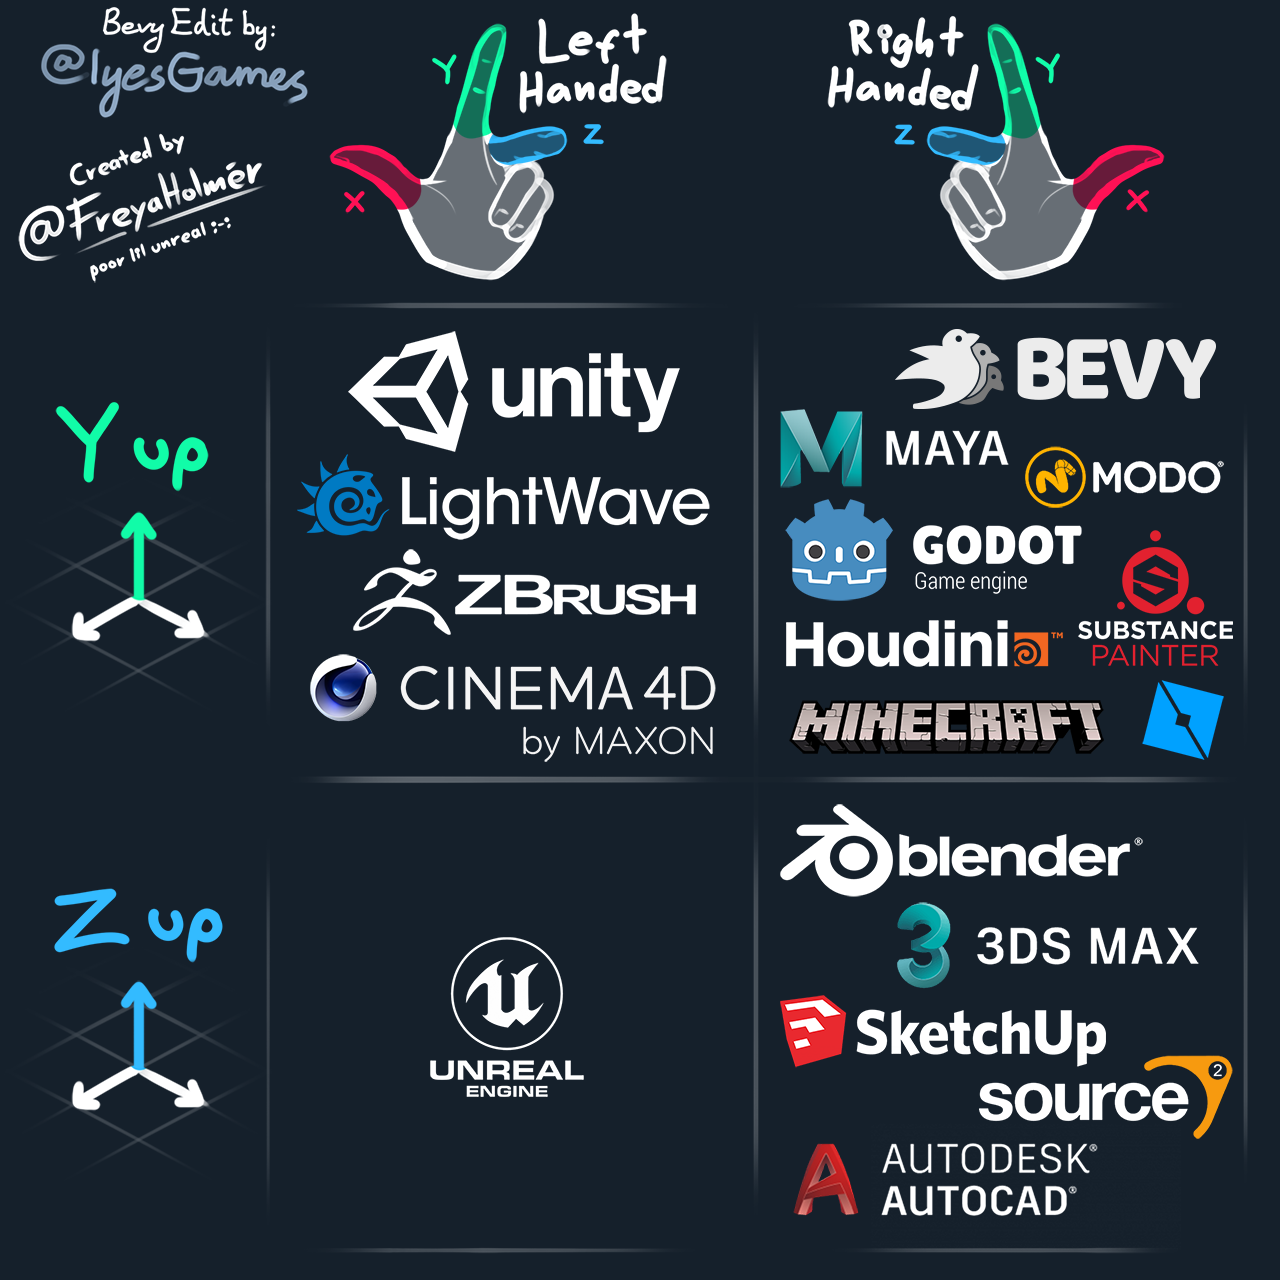
\includegraphics[width=0.8\textheight]{assets/3D_soft_handedness.png}
	\caption*{\url{https://bevy-cheatbook.github.io/fundamentals/coords.html}}
\end{figure}
\end{frame}

\begin{frame}
	\frametitle{Forward, up, right vectors}
	Which vectors are considered forward, upward, rightward, leftward, etc.?
	% \begin{figure}
	%     \centering
	%     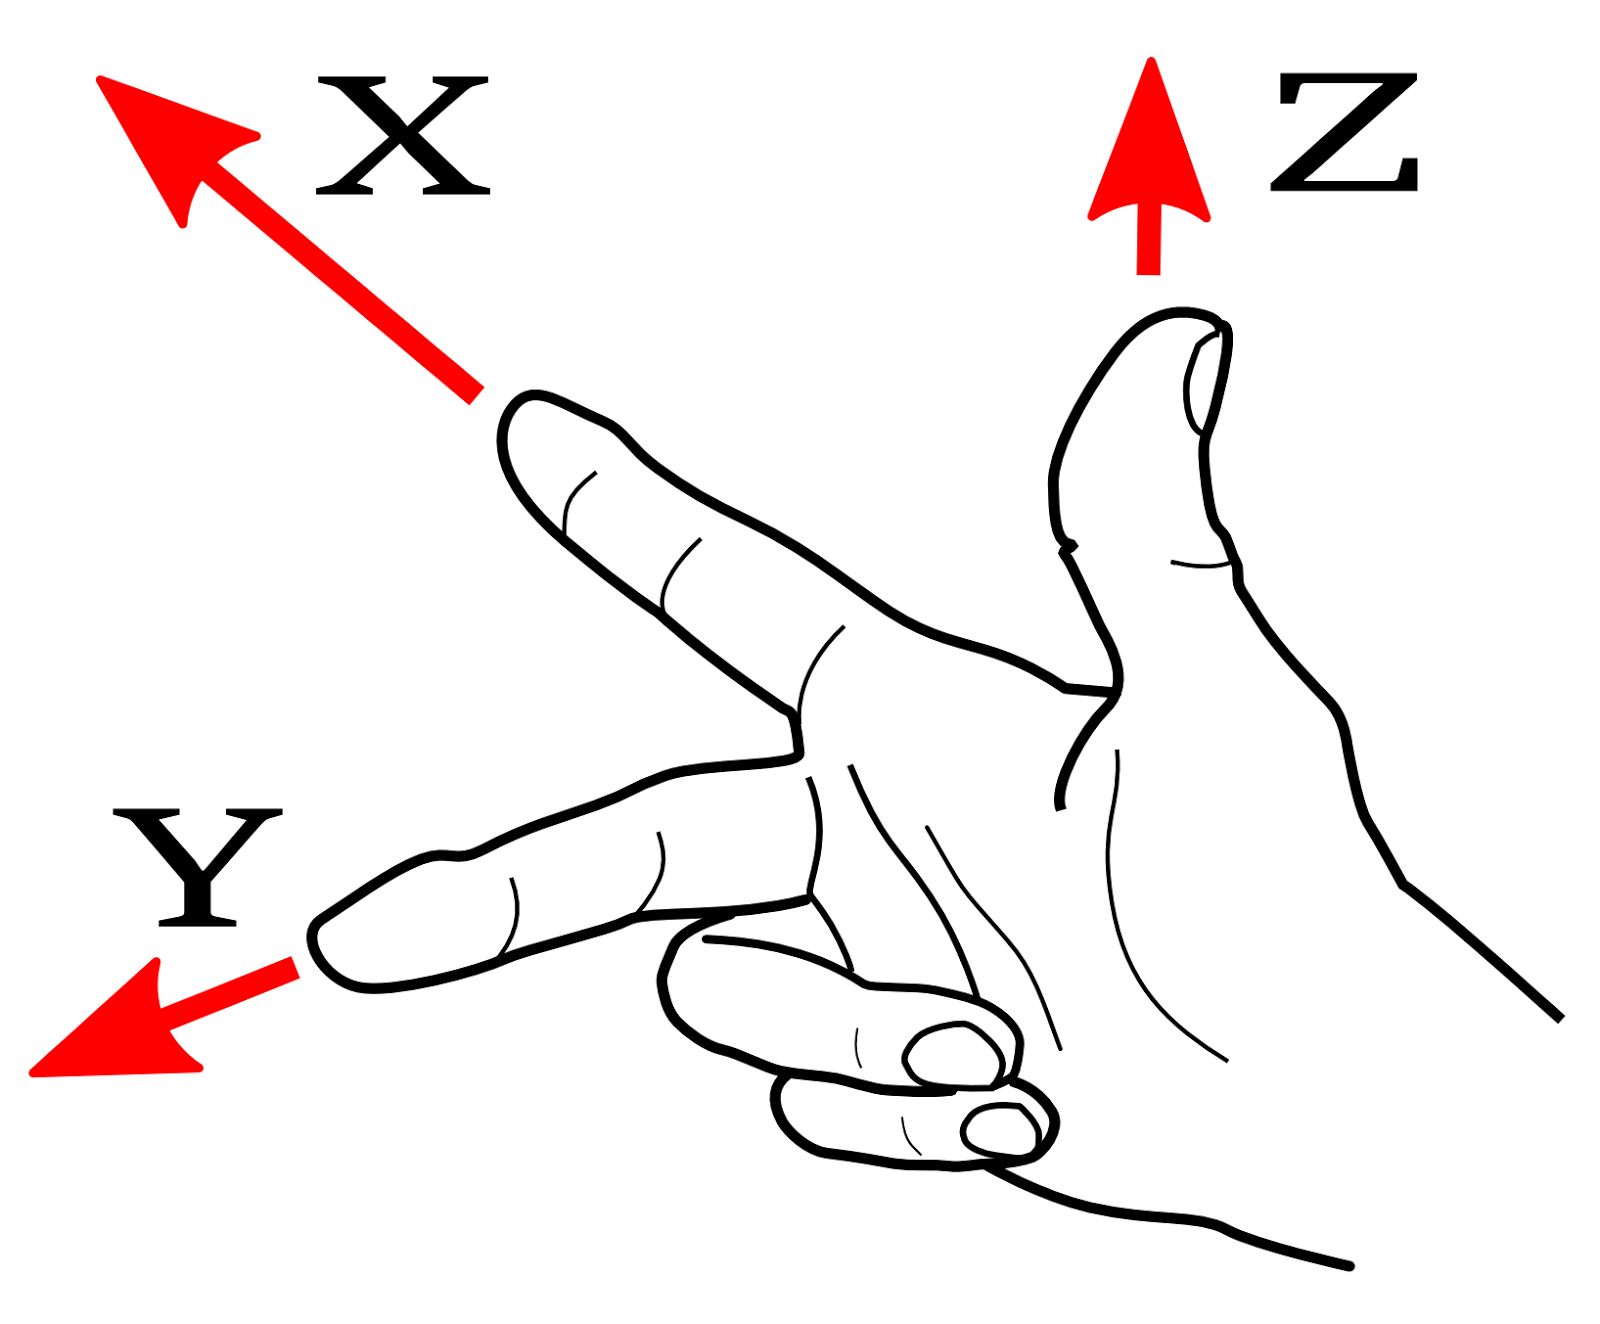
\includegraphics[width=0.5\textheight]{assets/fingers.png}
	% 	\caption*{\url{https://stackoverflow.com/a/34068511}}
	% \end{figure}
	\vfill
	This is pretty arbitrary: In 3D software it's pretty obvious which vector is considered the up vector. However, it's not obvious which vectors are the forward and right vectors. 
	\vfill
	Cameras, bones and regular geometry often have different coordinate systems from each other. 
\end{frame}

\begin{frame}
\frametitle{Positive angle}
Is positive angle clockwise or counterclockwise when viewing from the tip of the arrow towards the origin?
\begin{figure}
    \centering
    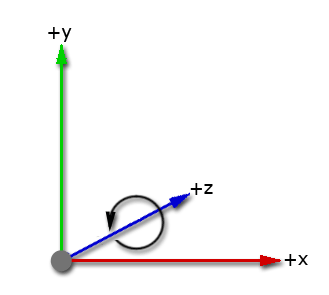
\includegraphics[width=0.7\textheight]{assets/unity-axis-with-rotation_positive_angle.png}
	\caption*{\url{https://docs.unity3d.com/Manual/QuaternionAndEulerRotationsInUnity.html}}
\end{figure}
\end{frame}



\begin{frame}
\frametitle{Intrinsic and extrinsic rotations}
When it comes to Euler angles, are rotations performed around global/parent axes (\textbf{extrinsic} rotations) or some local/child axes (\textbf{intrinsic} rotations)?
\vfill 	
See the pictures for a visual explanation:
\url{https://en.wikipedia.org/w/index.php?title=Davenport_chained_rotations&oldid=1222677779\#Conversion_between_intrinsic_and_extrinsic_rotations}
\vfill 	
Briefly stated, the order of axes gets reversed. For example, extrinsic XYZ order is the same thing as intrinsic ZYX order. 
\end{frame}

\begin{frame}
\frametitle{Matrix transposition}
Are 4x4 transformation matrices (that represent the rotation, translation and scaling of a 3D object) written like this
$$
\begin{bmatrix}
\mathbf{RS} & \vv{t} \\
\vv{0} & 1	
\end{bmatrix}
$$
or like this
$$
\begin{bmatrix}
\mathbf{(RS)}^\top & \vv{0}^\top \\
\vv{t}^\top & 1
\end{bmatrix}
$$
where $\mathbf{R}$ is a 3x3 rotation matrix,  $\mathbf{S}$ is a 3x3 scaling matrix, $\vv{t}$ is a 3x1 translation vector, and $\vv{0}$ is a 3x1 zero vector? In other words, are the matrices transposed or not? 
\vfill
This choice determines how vectors are transformed by matrices: they are either premultiplied ($\vv{v'}=\mathbf{R}\vv{v}$) or postmultiplied ($(\vv{v'})^\top=\vv{v}^\top\mathbf{R}^\top$). 
\end{frame}

\begin{frame}
\frametitle{Matrix transposition}
\begin{figure}
	\centering
	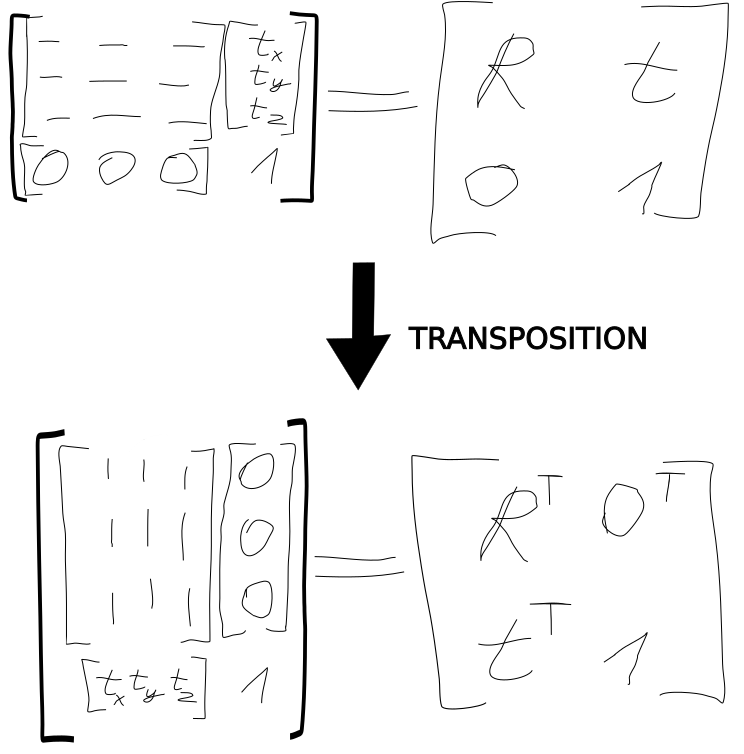
\includegraphics[width=0.8\textheight]{assets/transformation_matrix_transposition.png}
\end{figure}
\end{frame}

%##################################################################################

\section{Mathemtical representations}


\begin{frame}
\frametitle{2D rotations}
\begin{itemize}
	\item 2D (2x2) rotation matrices
	\begin{equation*} 
		\vecsymb{v}^{\prime} = \rotmatII{\theta} \vecsymb{v}
	\end{equation*}
	where $\theta$ is the angle of rotation, $\vv{v}$ is a vector before rotation, and $\vv{v}^\prime$ is the rotated vector.

	\item complex numbers 
	\begin{equation*}
		(x'+iy') = e^{i\theta}(x+iy) = (\complexnumb{\cos\theta}{\sin{\theta}})(x+iy).
	\end{equation*}
	where $\theta$ is the angle of rotation, $x$ and $y$ are the coordinates of a 2D vector before rotation, and $x'$ and $y'$ are the rotated coordinates.
\end{itemize}
Contrary to 3D rotations, 2D rotations are \textbf{commutative}!
\end{frame}


\begin{frame}
\frametitle{Euler angles}
3-tuple of angles (usally expressed in degrees, not radians) that express a sequence of 3 rotations around 3 perpendicular axes. 
\vfill
While not common in Compute Graphics, the first and third axes can be the same as in ZYZ, ZXZ, XYX, XZX, YZY, and YXY orders. 
\vfill
The order is important: ZYX is not equivalent to YZX. As mentioned before, intrinsic XYZ order is not the equivalent to extrinsic XYZ order. 
\vfill
All in all, there are 24 possible types of Euler angles.
\end{frame}

\begin{frame}
\frametitle{Euler angles $+/-$}
Upsides:
\begin{itemize}
	\item Intuitive when expressed relative to world/global coordinate system.
	\item Good for GUIs---only 3 numbers with no constraints (like unit-length or orthonormality constraints).
	\item Immune to gimbal lock, when only manipulating 2 angles.
\end{itemize}
Downsides:
\begin{itemize}
	\item Hard to compose (element-wise addition produces incorrect result).
	\item Very ambiguous (one rotation corresponds to many Euler angles, even of the same order).
	\item Hard to visualize.
	\item Experience gimbal lock.
	\item Not self-reliant---must be converted to other representations often.
	\item Without explicitly stating the order, bare 3-tuple is meaningless.
\end{itemize}	
\end{frame}


\begin{frame}
\frametitle{3D rotation matrices: X,Y,Z rotations}

To rotate around the X, Y, and Z axes, use the following matrices:
\[
\rotmat{\grotaxis{x}}{\theta} = 
\begin{bmatrix}	
	1 & 0 & 0 \\
	0 & \cos\theta & -\sin\theta\\
	0 & \sin\theta & \cos\theta
\end{bmatrix}
\]

\[
\rotmat{\grotaxis{y}}{\theta}  = 
\begin{bmatrix}	
	\cos\theta &  0&\sin\theta\\
	0 & 1 & 0 \\
	-\sin\theta & 0 & \cos\theta
\end{bmatrix}
\]

\[
\rotmat{\grotaxis{z}}{\theta} = 
\begin{bmatrix}	
	 \cos\theta & - \sin\theta & 0\\
	 \sin\theta & \cos\theta & 0 \\
	 0&0&1
\end{bmatrix}
\]
where $\theta$ is a rotation angle. 
Sometimes you might see them transposed (with the minus sign on the opposite side of the diagonal).

\end{frame}
	



\begin{frame}
\frametitle{3D rotation matrices: Euler-angles-like}

Extrinsic XYZ Euler angles can be represented as a rotation matrix by subsequently multiplying\footnote{
	Search for "matrix multiplication" in Google Images.
} the three rotation matrices for X, Y, and Z axes, in that order:
\begin{equation*} 
	\rotmat{\grotaxis{Z}}{\alpha} \rotmat{\grotaxis{Y}}{\beta} \rotmat{\grotaxis{X}}{\theta} =
		\begin{bmatrix} 
		c_{\alpha}c_{\beta}&{{c_{\alpha}s_{\beta}s_{\theta}-c_{\theta}s_{\alpha}}}&{{s_{\alpha}s_{\theta}+c_{\alpha}c_{\theta}s_{\beta}}}\\
		c_{\beta}s_{\alpha}&{{c_{\alpha}c_{\theta}+s_{\alpha}s_{\beta}s_{\theta}}}&{{c_{\theta}s_{\alpha}s_{\beta}-c_{\alpha}s_{\theta}}}\\
		-s_{\beta}&c_{\beta}s_{\theta} & c_{\beta}c_{\theta}
	\end{bmatrix}
\end{equation*} 
where $c_?=\cos(?)$ and $s_?=\sin(?)$. Angles are in radians, not degrees.
\vfill
There are 12 such Euler-angles-like rotation matrices. Why not 24? Because the extrinsic XYZ matrix is equivalent to the instrinsic ZYX matrix, etc.
\vfill

Rotations performed by such matrices are still prone to gimbal lock!
\end{frame}

\begin{frame}
\frametitle{3D rotation matrices: axis-angle-like}
A matrix that rotates $\theta$ radians around a vector $\rotaxisn$ is as follows:
\begin{equation*}\label{matrix:angle_axis_form}
	\rotmat{\rotaxis{n}}{\theta}
	{	\footnotesize
		=\begin{bmatrix}
			c+(n_1)^2(1-c)&n_1n_2(1-c)-sn_3&n_1n_3(1-c)+sn_2\\
			n_2n_1(1-c)+sn_3&c+(n_2)^2(1-c)&n_2n_3(1-c)-sn_1\\
			n_3n_1(1-c)-sn_2&n_3n_2(1-c)+sn_1&c+(n_3)^2(1-c)
	\end{bmatrix}}	
\end{equation*}
where $c=\cos\theta$ and $s=\sin\theta$. 
It can be verified that $\rotmat{\rotaxis{n}}{\theta}$ is indeed a rotation matrix around $\rotaxis{n}$ by confirming that 
$$
\rotmat{\rotaxis{n}}{\theta}\rotaxisn = \rotaxisn
$$ 
\vfill
Note that $\rotmat{\rotaxis{n}}{\theta} = \rotmat{\rotaxis{-n}}{-\theta}$.
\vfill
Rotations using this matrix are immune to gimbal lock!
\end{frame}

\begin{frame}
	\frametitle{3D rotation matrices: visualization}
	Assuming that all vectors are represented as column vectors, then 3D rotation matrices are simply containers for the X, Y and Z axes   
$$
\begin{bmatrix}
	\vert & \vert & \vert \\
	\grotaxis{x}   & \grotaxis{y}   &  \grotaxis{z}\\
	\vert & \vert & \vert
\end{bmatrix}.
$$
This is extremely useful for visualization and debugging. 
\end{frame}

\begin{frame}
	\frametitle{3D rotation matrices: Rodriguez formula}
	Without any effort, $\rotmat{\rotaxis{n}}{\theta}$ can be decomposed into the following sum:
	\begin{equation*} 
		\rotmat{\rotaxis{n}}{\theta} = (\cos\theta) \mathbf{I} + (\sin\theta) \crossmat{\rotaxis{n}} + (1-\cos\theta)(\rotaxis{n}\rotaxis{n}^\top)
	\end{equation*}
	where $\crossmat{\rotaxis{n}}$ is the cross product matrix of $\rotaxis{n}$:
	$$
	\crossmat{\rotaxis{n}} = \crossmatfull{n_1}{n_2}{n_3},
	$$
	and $\rotaxis{n}\rotaxis{n}^\top$ is as follows:
	$$
	\rotaxis{n}\rotaxis{n}^\top = \begin{bmatrix}
					n_1^2&n_1n_2&n_1n_3\\
		n_2n_1&n_2^2&n_2n_3\\
		n_3n_1&n_3n_2&n_3^2.
	\end{bmatrix}
	$$
	This formula is known as the \textit{Euler-Rodriguez formula} for rotation matrices.
	Equivalently, it can be reformulated as:
	$$
		\rotmat{\rotaxis{n}}{\theta} =  I + (sin\theta) \crossmat{\rotaxis{n}} + (1-\cos\theta)\crossmat{\rotaxis{n}}^2.
	$$
	\end{frame}

\begin{frame}
\frametitle{3D rotation matrices $+/-$ (SPOILER: they are the best)}
Upsides:
\begin{itemize}
	\item Easy to visualize!
	\item Immune to gimbal lock\footnote{When not performing sequential rotations around mutually prpendicular axes (like in Euler angles)!}.
	\item Non-ambiguous: one rotation corresponds to exactly one matrix. 
	\item Probably benefit from CPU and GPU optimizations for matrix multiplication (speculating).
\end{itemize}
Downsides:
\begin{itemize}
	\item Need to store 9 numbers.
	\item Need to reorthogonalize to prevent numerical errors from accumulating (speculating). 
\end{itemize}
\end{frame}

\begin{frame}
\frametitle{Unit-length quaternions}
Don't try to visualize them in 3D space. Just learn their algebraic rules: how to multiply them, how to invert them, how to normalize them, etc. Also, learn how to extract axis and angle from them. 
\vfill
Not every quaternion represents a rotation: only the unit-length ones!
\vfill 
Quaternion $q$ can be represented   as a sum of the scalar part and the imaginary parts or as a tuple consisting of a scalar and a vector:
$$
q = q_0 + iq_1 + jq_2 + kq_3 = (q_0, \mathbf{q}) = (q_0, q_1, q_2, q_3) = (q_0, (q_1, q_2, q_3)),
$$
where $q_0$ is the scalar part and $\mathbf{q} = (q_1, q_2, q_3)$ is the vector part.
Often, $q_0$ is called $w$ and $(q_1, q_2, q_3)$ is called $(x,y,z)$.
\end{frame}

\begin{frame}
\frametitle{Unit-length quaternions: rotations}
The four components of a unit quaternion can also be represented as
\begin{equation*}
q = \textstyle(\cos\frac{\theta}{2} , \rotaxis{n}\sin\frac{\theta}{2}),
\end{equation*}
where $\rotaxis{n}$ is the axis of rotation and $\theta$ its angle in radians ($\frac{\theta}{2}$ is not the angle of rotation!).
\vfill
To rotate a quaternion $q_1$ by a quaternion $q_2$, simply multiply them to obtain some quaternion $q_3$:
$$
q_3 = q_2 * q_1
$$
\vfill
To rotate a 3D vector $\vecsymb{v}$ by a quaternion $q$, treat $\vecsymb{v}$ as a quaternion with scalar part equal to 0 (such quaternions are called \textit{pure quaternions}), and multiply it from both sides:
$$
\quatvec{0}{\vecsymb{v}'} = q * \quatvec{0}{\vecsymb{v}} * q^{-1} 
$$
The right hand side can be expanded in such a way as to reveal the Euler-Rodriguez formula.  
\end{frame}

\begin{frame}
\frametitle{Unit-length quaternions $+/-$}
Upsides:
\begin{itemize}
	\item Need to store only 4 numbers.
	\item Immune to gimbal lock\footnote{When not performing sequential rotations around mutually prpendicular axes (like in Euler angles)!}.
	\item Allow rotating around an arbitrary axis.
	\item Straightforward to derive $SLERP$ and $NLERP$. 
	\item Normalizing quaternions after each multiplication prevents numerical errors from accummulating (speculating). 
\end{itemize}
Downside:
\begin{itemize}
	\item Ambiguous: quaternion $q$ represents the same rotation as $-q$.
	\item Hard to visualize.
	\item Seem scary to non-maths people.
	\item Store only rotation whereas 4x4 transformation matrices can additionally store translation and scaling.
\end{itemize}
\end{frame}
    

\begin{frame}
\frametitle{Axis-angle}
Probably the simplest way to represent a rotation around some axis $\rotaxis{n}$ and an angle $\theta$ is using either a tuple
$$
\left(\begin{bmatrix}
n_1 \\
n_2 \\
n_3	
\end{bmatrix}, \theta\right) 
$$
or a vector
$$
	\theta \begin{bmatrix}
	n_1 \\
	n_2 \\
	n_3	
\end{bmatrix}.
$$
For example, a $\degree{45}$ rotation around an axis halfway between the $\grotaxis{X}$ and $\grotaxis{Z}$ axes is as follows:
$$
\frac{\pi}{4} \begin{bmatrix}
	\frac{1}{\sqrt{2}}  \\
	0 \\
	\frac{1}{\sqrt{2}}
\end{bmatrix}
$$
\end{frame}



\begin{frame}
\frametitle{Axis-angle: exponential map}
Axis-angle vectors and tuples can't be composed on their own: a sum or a dot product\footnote{Search for "vector dot product" in Google.} produce incorrect results.
To address this, we define functions $\exp$ and $\log$.
\vfill
$\exp$ converts axis-angle vectors to quaternions or rotation matrices.
$\log$ converts quaternions or rotation matrices back to axis angle vectors.
\vfill
They are useful for calculating derivatives\footnote{The derivative of a function measures how the function is changing (how fast, in which direction, etc.)} of functions involving rotations. There is a deep theory behind these functions, but it's not something 3D animators need to know.
\end{frame}
    
\begin{frame}
\frametitle{Axis-angle $+/-$}
Upsides:
\begin{itemize}
	\item Intuitive.
	\item Only 3 numbers to store.
	\item Cool for calculating derivatives (tbh, I don't know much about it). 
	\item $\exp$ and $\log$ map make it easy to generalize $SLERP$ to rotation matrices. 
\end{itemize}
Downsides:
\begin{itemize}
	\item Not self-reliant---must be converted to other representations often.
	\item $\rotaxisn \theta$ express the same rotation as $(-\rotaxisn)(-\theta)$.
	\item Maybe they are necessary for some things, but I'm not advanced enough to know about it and fully appreciate it. (haha)
\end{itemize}
\end{frame}

\begin{frame}
\frametitle{In SciPy}
\url{https://docs.scipy.org/doc/scipy/reference/generated/scipy.spatial.transform.Rotation.as_quat.html}
\vfill
Note the \hl{seq} argument in \hl{as\_euler} method. Also note the \hl{canonical} and \hl{scalar\_first} arguments in \hl{as\_quat}.
\vfill
We didn't cover: 
\begin{itemize}
	\item Davenport angles --- like Euler angles but generalized to nonperpendicular axes.  
	\item Modified Rodriguez Parameters (MRP) --- like axis-angle vectors but the angle of rotation is transformed.
\end{itemize}
\end{frame}

%##################################################################################

\section{Miscellaneous}


\begin{frame}
\frametitle{Gimbal lock}
Tbh, I don't know the full theory behind gimbal lock. Most of the sources seem to only give examples of when gimbal lock happens. Don't take my word for what I'm about to say.
\vfill
Basically, for some special values of Euler angles, two angles rotate around the same axis.
\vfill
For the 3 perpencidular axes Euler angles (XYZ, ZXY, YZX, etc.), it happens when the middle angle is set to $\pm\degree{90}$. 
\vfill
For the 2 perpendicular axes Euler angles (XYX, ZYZ, YZY, etc.), it happens when the middle angle is set to $\degree{0}$ or $\pm\degree{180}$.
\vfill
In gimbal lock, small changes of axis-angle parametrized functions result in huge changes in Euler angles.
\end{frame}


\begin{frame}
\frametitle{A-to-B rotation interpolation: SLERP}
You provide two keyframes at A and B; the inbetween frames are interpolated by the 3D software. Let's focus on quaternions.
\vfill
$SLERP$ (\textit{spherical linear interpolation}) is the proper way to interpolate two quaternions: the "movement" it produces has constant angular velocity, and follows the shortest path.
\begin{equation*} 
SLERP(q_0, q_1, t) = 
\frac{\sin((1-t)\theta)}{\sin(\theta)}q_0 + \frac{\sin(t\theta)}{\sin(\theta)}q_1 
\end{equation*}
Surprisingly, $SLERP(q_0, q_1, t)$ and $SLERP(-q_0, q_1, t)$ produce different results.
\end{frame}

\begin{frame}
	\frametitle{A-to-B rotation interpolation: NLERP}
$NLERP$ (\textit{normalized linear interpolation}) is faster and easier to compute. It follows the same path as $SLERP$, but the angular velocity is not constant\footnote{But it's not bad. Blender uses $NLERP$ by default for rotation interpolation.}. Basically, it computes $LERP$ on two quaternions and normalizes the result so that the unit-length constraint is satisfied. 
\vfill
Simple $LERP$ is defined as follows:
\begin{align*}
	LERP(q,p,t) = (&q_0(1-t) + p_0t, \\
	(&q_1(1-t) + p_1t, \\
	&q_2(1-t) + p_2t, \\
	&q_3(1-t) + p_3t )),
\end{align*}
where $t \in [0,1]$ and $q$ and $p$ are some unit-length quaternions. Then, $NLERP$ is defined as
 $$
NLERP(q,p,t) = 
\frac{LERP(q,p,t)}{\norm{LERP(q,p,t)}}.
$$
\end{frame}


\begin{frame}
\frametitle{A-to-C-through-B rotation interpolation}
\begin{figure}
    \centering
    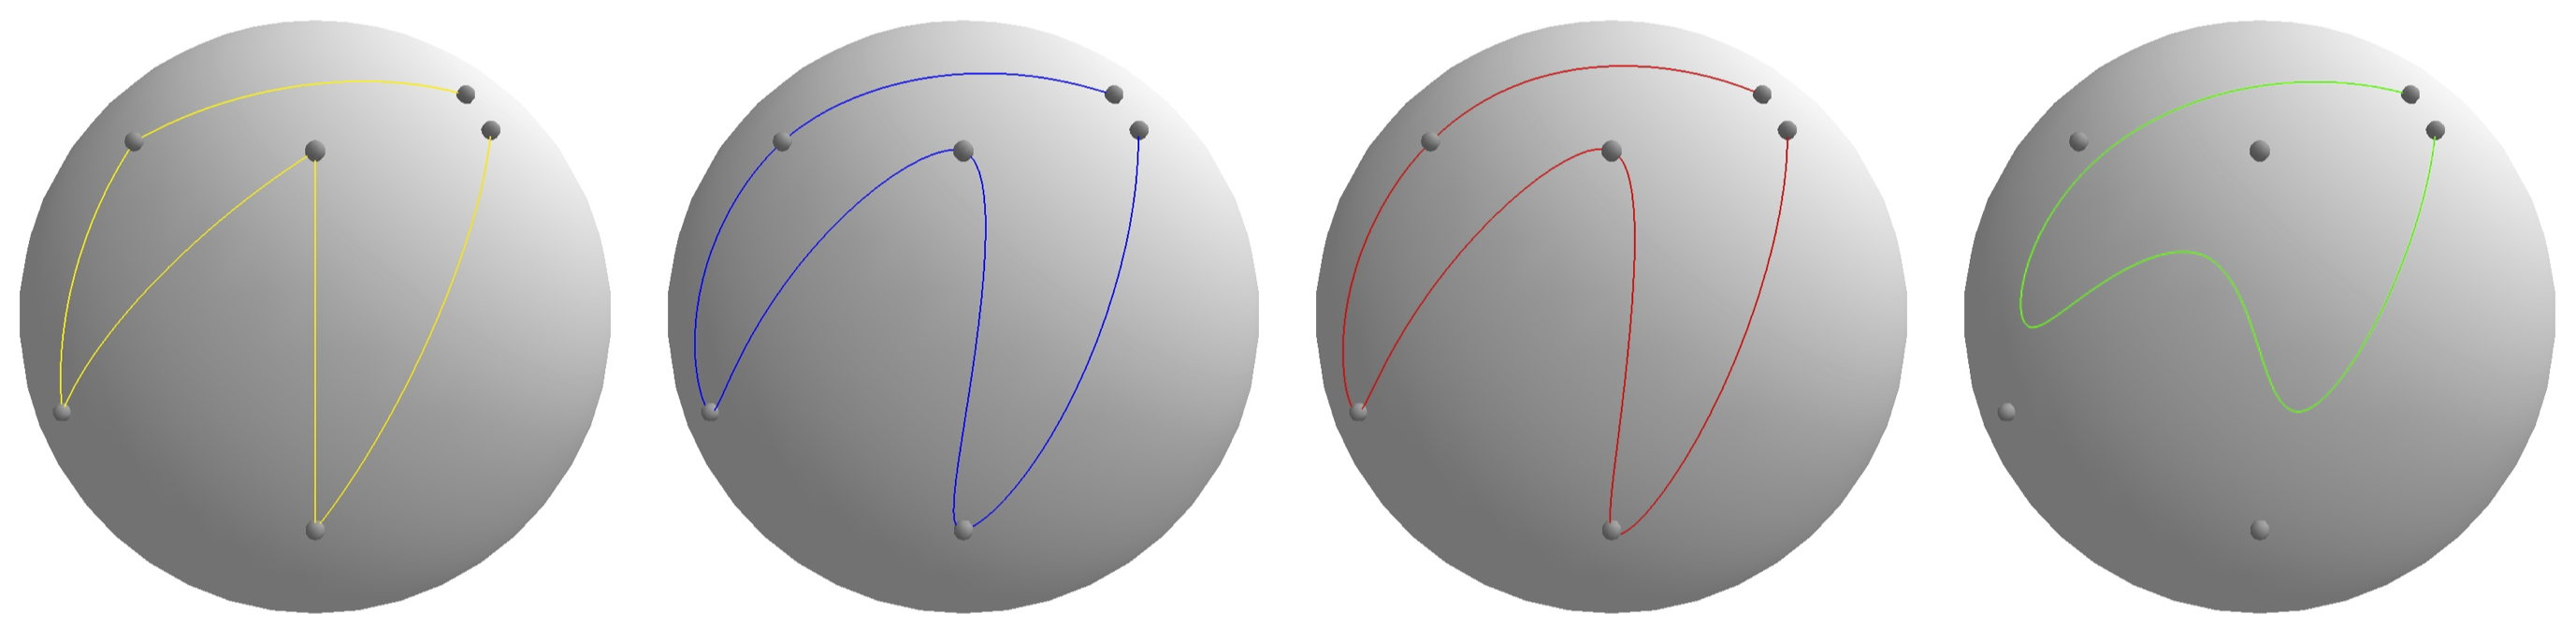
\includegraphics[width=1\textwidth]{assets/higher_order_interp_orientation.png}
	\caption*{\url{https://www.adrian-haarbach.de/interpolation-methods/}}
\end{figure}

\end{frame}



%##################################################################################

\end{document}

%##################################################################################
